\chapter{Analysis of Parasite Clearance Times}
\begin{table}[h]
\centering
\caption{Derived PC90 values}\label{pc90}
\begin{tabular}{|cc|c|c|}
\hline
&&\multicolumn{2}{c|}{Treatment}\\
Centre&Sex&A&B\\\hline
\multirow{2}{*}{001}&M&$\begin{array}{c}3.8,\ 27.9,\ 34.3,\  9.8,\\5.0,\  0.8,\ 28.9,\  4.7\end{array}$&$\begin{array}{c}9.5,\  5.3,\  7.7,\\23.5,\  9.4,\  8.1\end{array}$\\\cline{2-4}
&F&$\begin{array}{c}21.1,\ 23.2,\\22.5,\ 47.2\end{array}$&$\begin{array}{c}4.2,\ 8.6 ,\ 9.4,\\0.9,\ 8.6,\ 12.9\end{array}$\\\hline
\multirow{2}{*}{002}&M&$\begin{array}{c}4.5,\ 2.1,\\20.6,\ 29.1\end{array}$&$\begin{array}{c}19.3,\ 10.0,\\15.6,\ 8.9\end{array}$\\\cline{2-4}
&F&$\begin{array}{c}20.1,\ 2.2,\ 24.0,\ 28.7,\\5.0,\ 22.2,\ 23.7\end{array}$&$\begin{array}{c}15.4,\  8.4,\\5.9,\ 6.3\end{array}$\\\hline
\end{tabular}
\end{table}
\subsection{PC90 ANOVA} 
3-way ANOVA with interactions was performed on the PC90 data over centre, sex and treatment. The results are shown in Table \ref{anova}. It can be seen that the only significant effect on PC90 is the treatment used (\texttt{trt}), with perhaps some effect of the interaction between sex and treatment. This is a result we might expect. If we fit a model with treatment as the only factor we find that treatment B reduces the PC90 time compared to treatment A by 8.0 hours with a 95\% confidence interval of (1.9, 14.1) hours.
\begin{table}[h]
\centering
\caption{3-way ANOVA with interactions for PC90}\label{anova}
\begin{boxedverbatim}
Response: PC90
                                         Df Sum Sq Mean Sq F value  Pr(>F)  
factor(SEX)                               1   49.4    49.4  0.5218 0.47488  
factor(CENTREID)                          1    0.1     0.1  0.0008 0.97816  
factor(trt)                               1  697.5   697.5  7.3708 0.01022 *
factor(SEX):factor(CENTREID)              1   57.4    57.4  0.6062 0.44146  
factor(SEX):factor(trt)                   1  389.4   389.4  4.1151 0.05016 .
factor(CENTREID):factor(trt)              1  143.4   143.4  1.5150 0.22658  
factor(SEX):factor(CENTREID):factor(trt)  1   49.3    49.3  0.5214 0.47505  
Residuals                                35 3312.0    94.6
\end{boxedverbatim}
\end{table}

Diagnostic plots of the residuals of the ANOVA model are shown in Figure \ref{resid}. There does not seem to be any significant departure from normality in the distribution of residuals which suggests that we may not need a transformation for modelling the PC90 data. However, there is perhaps some evidence of heteroskedasticity in that the variance of the residuals appears to increase with increasing fitted PC90 value, hence we may need a variance-stabalising transformation.
\begin{sidewaysfigure}[p]
\centering
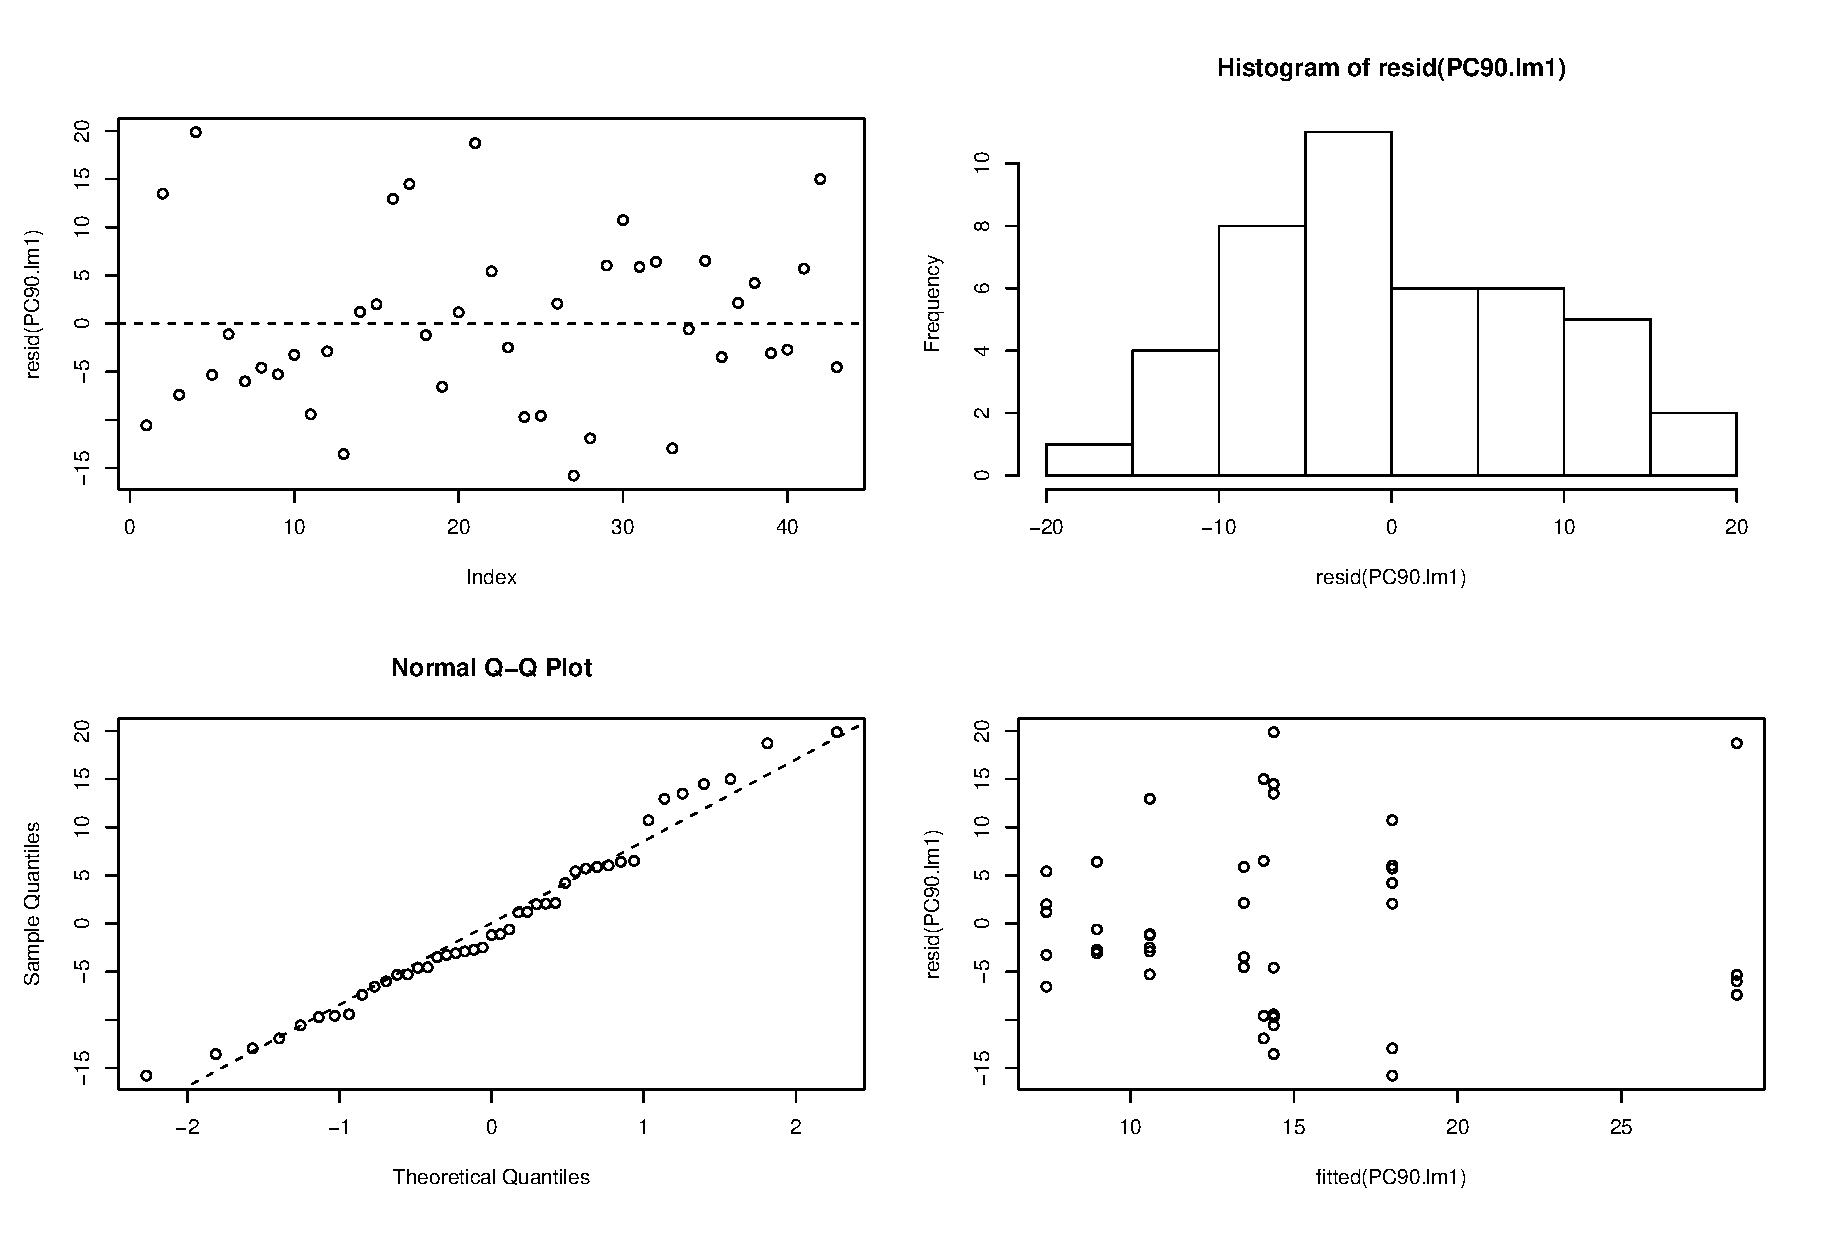
\includegraphics[scale=0.8]{PC90diag.eps}
\caption{Residuals for ANOVA on PC90}\label{resid}
\end{sidewaysfigure}

If we repeat the 3-way ANOVA of the previous report we find that \emph{Treatment} is the only factor that affects PC90 whichever method we use. Hence it would seem that the simplest method i.e. linear interpolation is the best method at this stage. However, as we know, the parasite count can be unreliable and depends on an operator-selected ``suitable" blood sample and so just one outlying value could throw the estimate by linear interpolation out as it only uses the two values above and below the PC90 count. In this respect an estimate based on more values should be more robust.

\subsection{ANCOVA}